\documentclass[tikz,border=5]{standalone}
\usepackage{tikz}
\usetikzlibrary{positioning}
\usepackage{eqnarray, amsmath}
\usepackage{xcolor}

\begin{document}

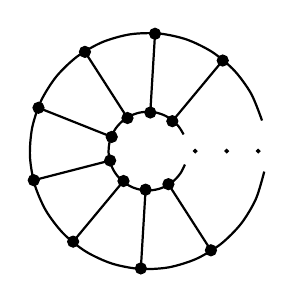
\begin{tikzpicture}
%CLOSE LADDER
%two basic circles
\draw[black, thick, domain=25:340] plot[smooth] ({0.5*cos(\x)}, {0.5*sin(\x)});
\draw[black, thick, domain=15:350] plot[smooth] ({1.5*cos(\x)}, {1.5*sin(\x)});
%dots
\filldraw[color=black, thin] (0.6,0) circle (0.65pt);
\filldraw[color=black, thin] (1.0,0) circle (0.65pt);
\filldraw[color=black, thin] (1.4,0) circle (0.65pt);
%points 1 circle
\filldraw[color=black] (0.31,0.38) circle (2pt);
\filldraw[color=black] (0.03,0.49) circle (2pt);
\filldraw[color=black] (-0.26,0.42) circle (2pt);
\filldraw[color=black] (-0.46,0.18) circle (2pt);
\filldraw[color=black] (-0.48,-0.12) circle (2pt);
\filldraw[color=black] (-0.31,-0.38) circle (2pt);
\filldraw[color=black] (-0.03,-0.49) circle (2pt);
\filldraw[color=black] (0.26,-0.42) circle (2pt);
%points 2 circle
\filldraw[color=black] (0.95,1.15) circle (2pt);
\filldraw[color=black] (0.09,1.49) circle (2pt);
\filldraw[color=black] (-0.80,1.26) circle (2pt);
\filldraw[color=black] (-1.39,0.55) circle (2pt);
\filldraw[color=black] (-1.45,-0.37) circle (2pt);
\filldraw[color=black] (-0.95,-1.15) circle (2pt);
\filldraw[color=black] (-0.09,-1.49) circle (2pt);
\filldraw[color=black] (0.80,-1.26) circle (2pt);
%connection lines
\draw[black, thick] (0.31,0.38) -- (0.95,1.15);
\draw[black, thick] (0.03,0.49) -- (0.09,1.49);
\draw[black, thick] (-0.26,0.42) -- (-0.80,1.26);
\draw[black, thick] (-0.46,0.18) -- (-1.39,0.55);
\draw[black, thick] (-0.48,-0.12) -- (-1.45,-0.37);
\draw[black, thick] (-0.31,-0.38) -- (-0.95,-1.15);
\draw[black, thick] (-0.03,-0.49) -- (-0.09,-1.49);
\draw[black, thick] (0.26,-0.42) -- (0.80,-1.26);
\end{tikzpicture}

\end{document}